\documentclass[10pt,a4paper]{article}
\usepackage{fontspec}
\setmainfont{Arial}
\usepackage[spanish,es-noshorthands]{babel}
\usepackage[a4paper,margin=1.8cm]{geometry}
\usepackage{amsmath,amssymb}
\usepackage{graphicx}
\usepackage{booktabs}
\usepackage{caption}
\usepackage{float}
\usepackage[hidelinks]{hyperref}
\graphicspath{{figuras_lazo/}}
\captionsetup{font=small,labelfont=bf}
\setlength{\parskip}{0.5em}
\setlength{\parindent}{0pt}

\title{Seguimiento de la referencia en lazo cerrado}
\date{}
\author{}

\begin{document}
\maketitle
\vspace{-12mm}

\section{Referencias}

\subsection{Theta-gamma con ventana}

Referencia:
\begin{align*}
r_I(t) &= T_w(t)\,\big[\,0{,}2\,\sin(2\pi f_\gamma t - 0{,}94) + 0{,}25\,\big],\\
r_E(t) &= T_w(t)\,\big[\,0{,}3\,\sin(2\pi f_\gamma t) + 0{,}45\,\big],\\
T_w(t) &= \begin{cases} 1 & \text{si } \big|\pi - |\varphi_\theta(t)|\big| < \pi/4,\\ 0 & \text{si no,} \end{cases}
\end{align*}
con $f_\gamma = 120$~Hz, $t \in [0, 2000]$~ms y $\varphi_\theta$ la fase de una theta de 4 a 12~Hz.

\begin{figure}[H]
\centering
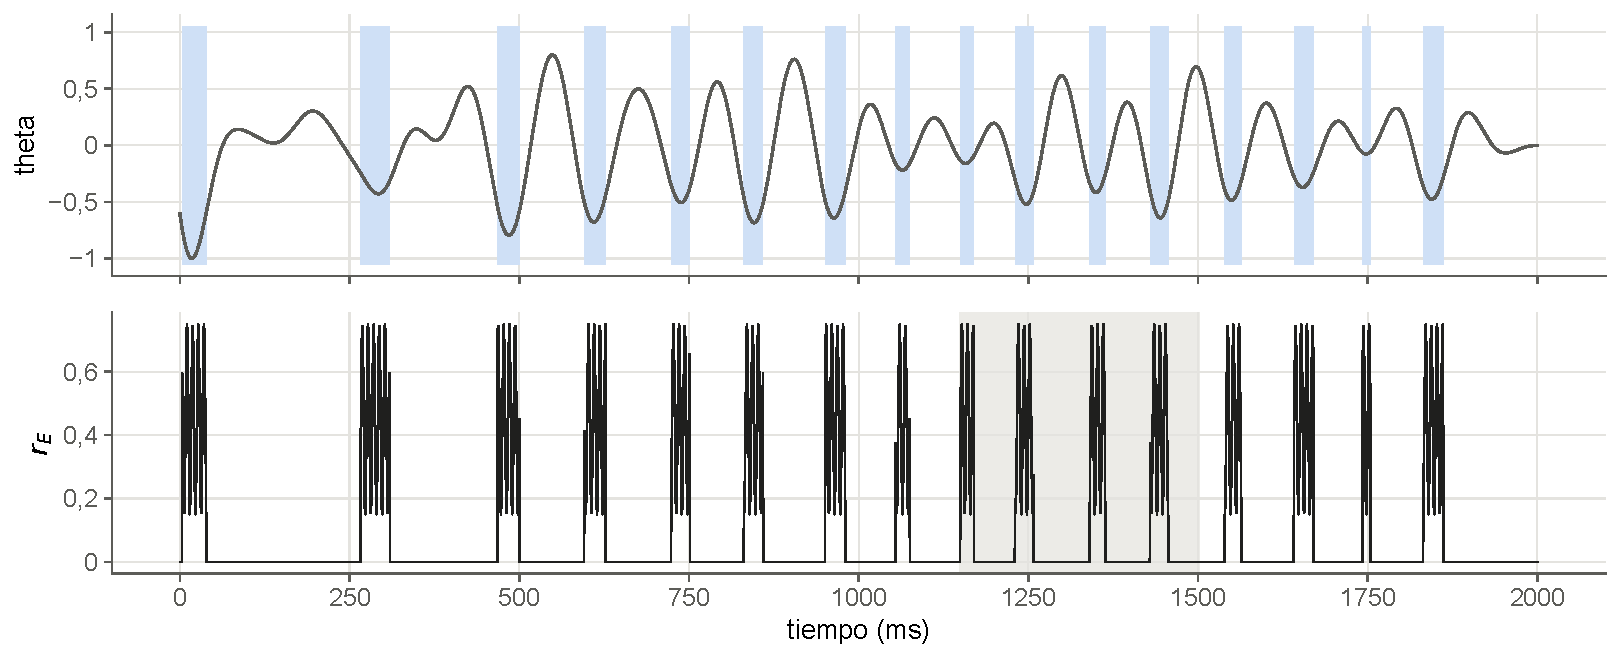
\includegraphics[width=\textwidth]{theta2s_referencia.pdf}
\caption{Arriba, la theta, con $T_w = 1$ en celeste. Abajo, $r_E$. En gris, la ventana de las figuras siguientes.}
\end{figure}

\begin{figure}[H]
\centering
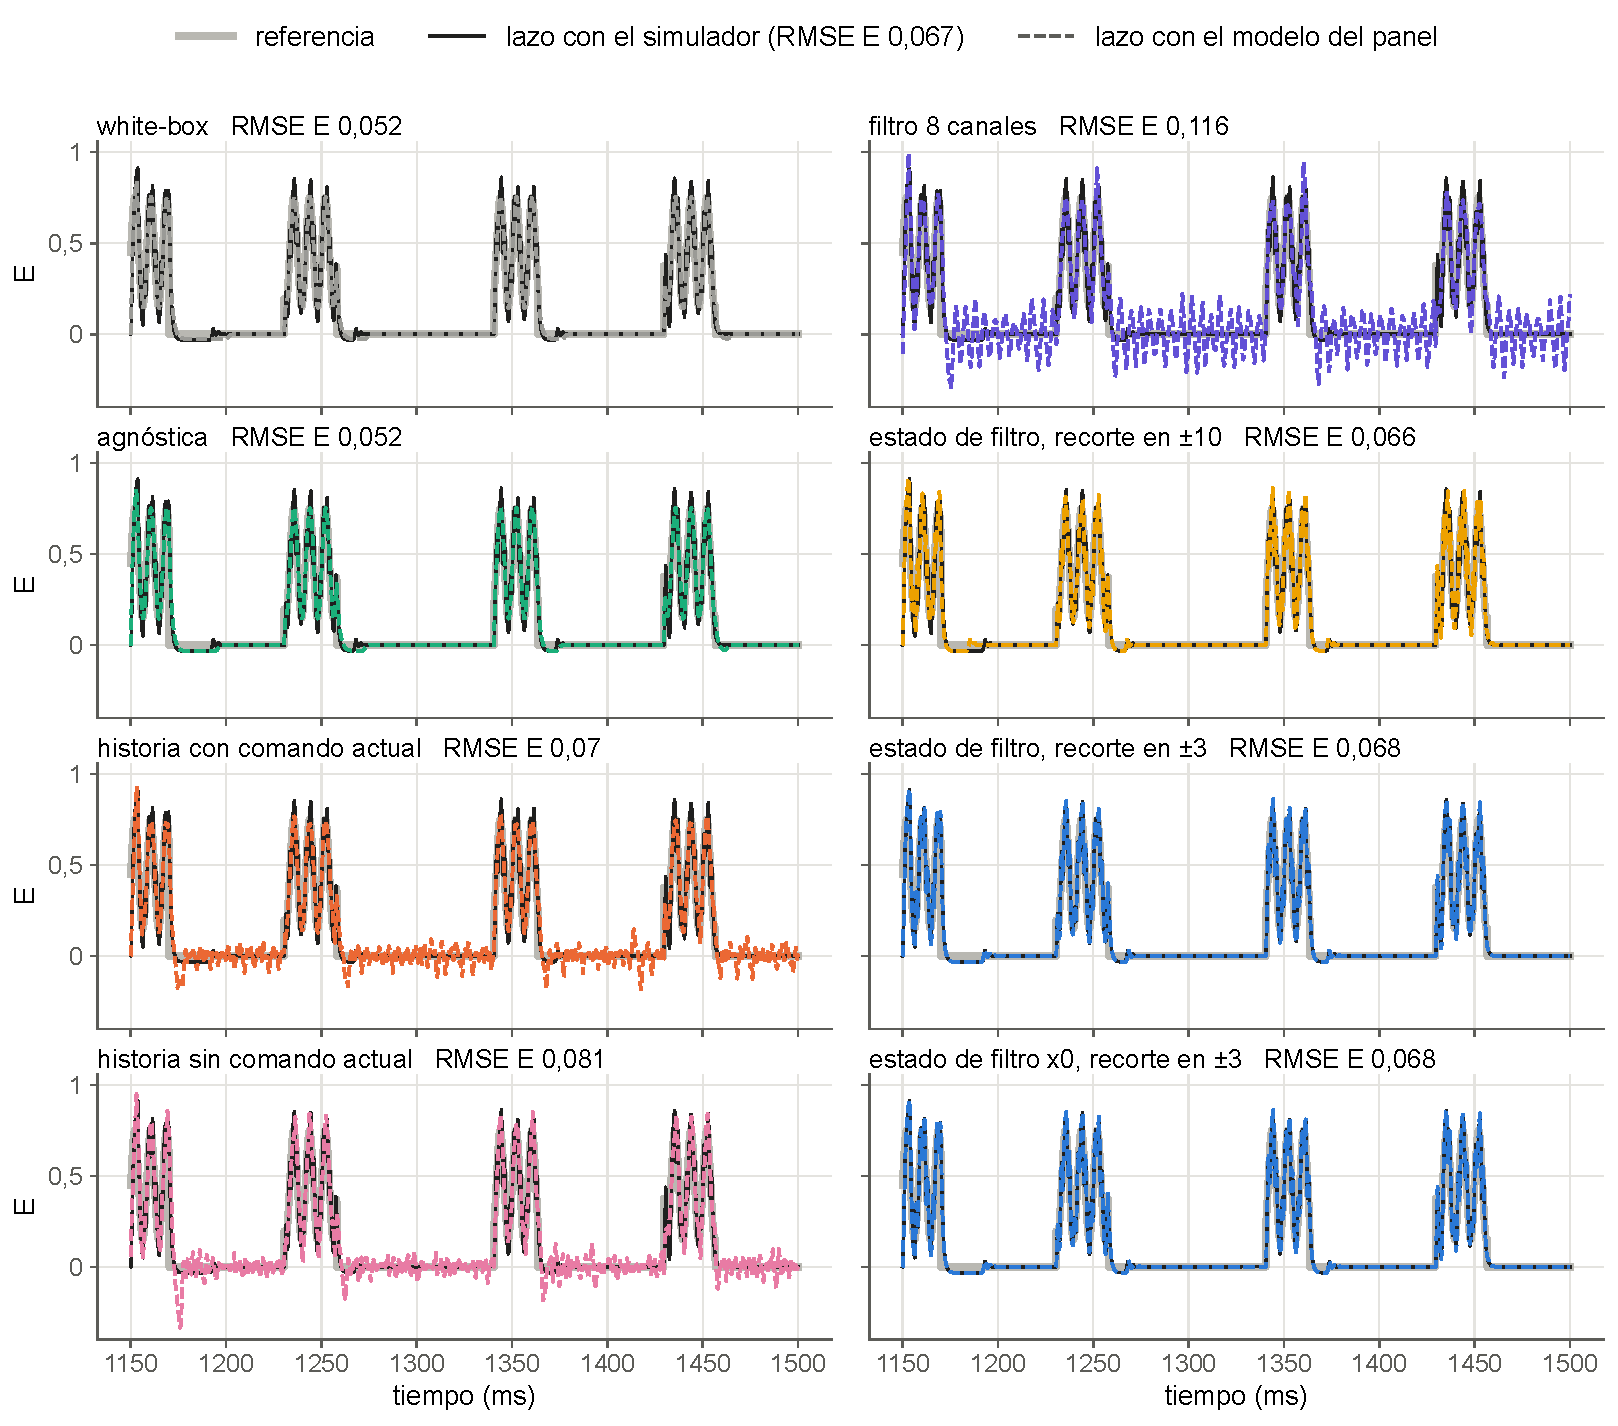
\includegraphics[width=\textwidth]{theta2s_E.pdf}
\caption{Actividad excitatoria $E$ con la referencia theta-gamma, entre 1150 y 1500~ms. Gris, referencia. Negro, lazo con el simulador. Discontinua, lazo con el modelo del panel.}
\end{figure}
\begin{figure}[H]
\centering
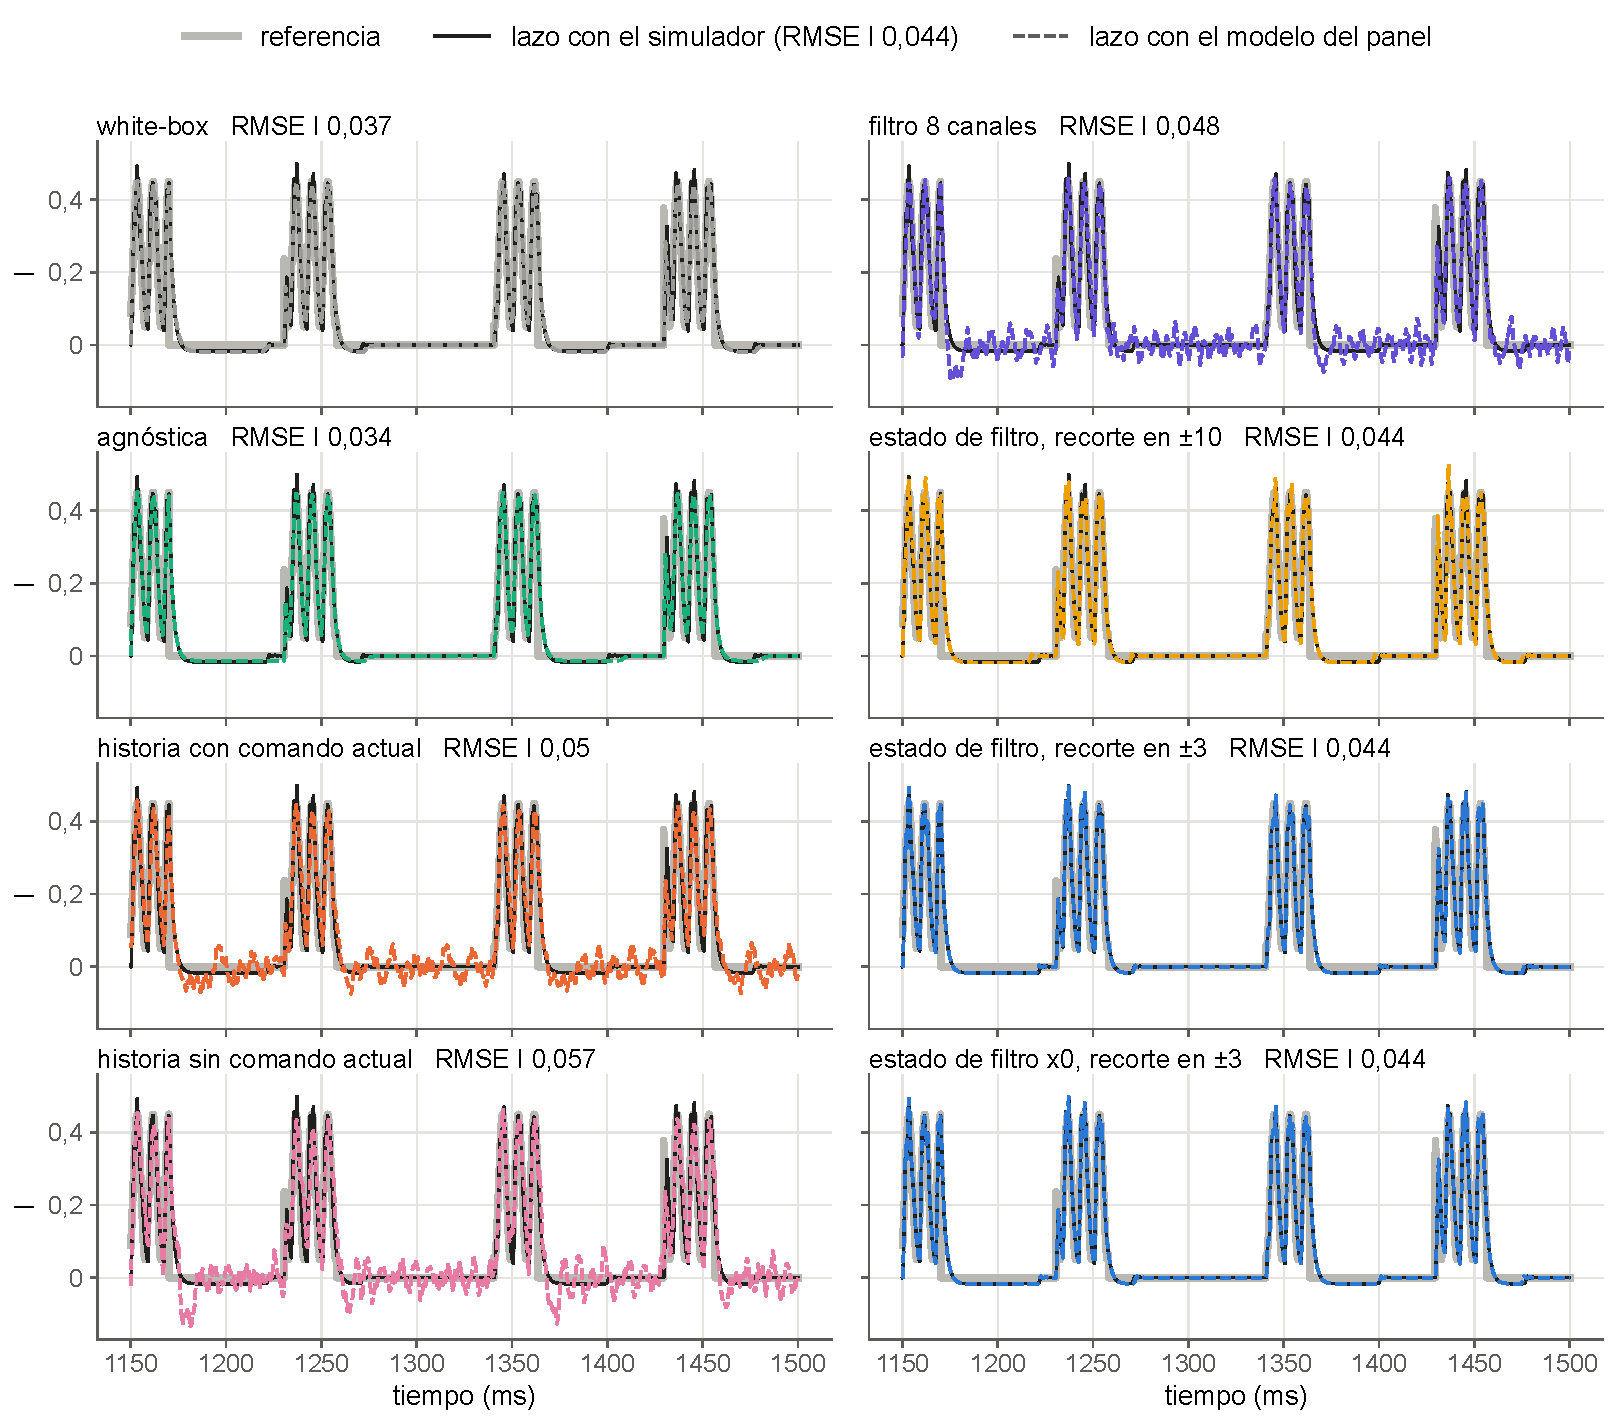
\includegraphics[width=\textwidth]{theta2s_I.pdf}
\caption{Actividad inhibitoria $I$ en las mismas corridas.}
\end{figure}
Dentro de cada ráfaga, el lazo con el simulador sigue la forma de la gamma con errores en los picos. El white-box y la agnóstica quedan más cerca de la referencia que el propio simulador (RMSE de $E$ 0,052 contra 0,067), porque el controlador invierte un Wilson-Cowan sin actuador y los cancela casi exactamente. El estado de filtro con recorte en $\pm 3$ se superpone al lazo con el simulador, con y sin x0 entrenable. Con recorte en $\pm 10$ se separa en los picos de algunas ráfagas. Las tres correcciones con historia del comando siguen las ráfagas, pero oscilan en los tramos de reposo entre ráfagas, donde la referencia y el lazo con el simulador valen cero. El filtro de 8 canales es el que más oscila (RMSE de $E$ 0,116).


\subsection{Gamma continua de 50~ms}

Referencia:
\begin{align*}
r_I(t) &= 0{,}2\,\sin(2\pi f_\gamma t - 0{,}94) + 0{,}25,\\
r_E(t) &= 0{,}3\,\sin(2\pi f_\gamma t) + 0{,}45,
\end{align*}
con $f_\gamma = 120$~Hz y $t \in [0, 50]$~ms.

\begin{figure}[H]
\centering
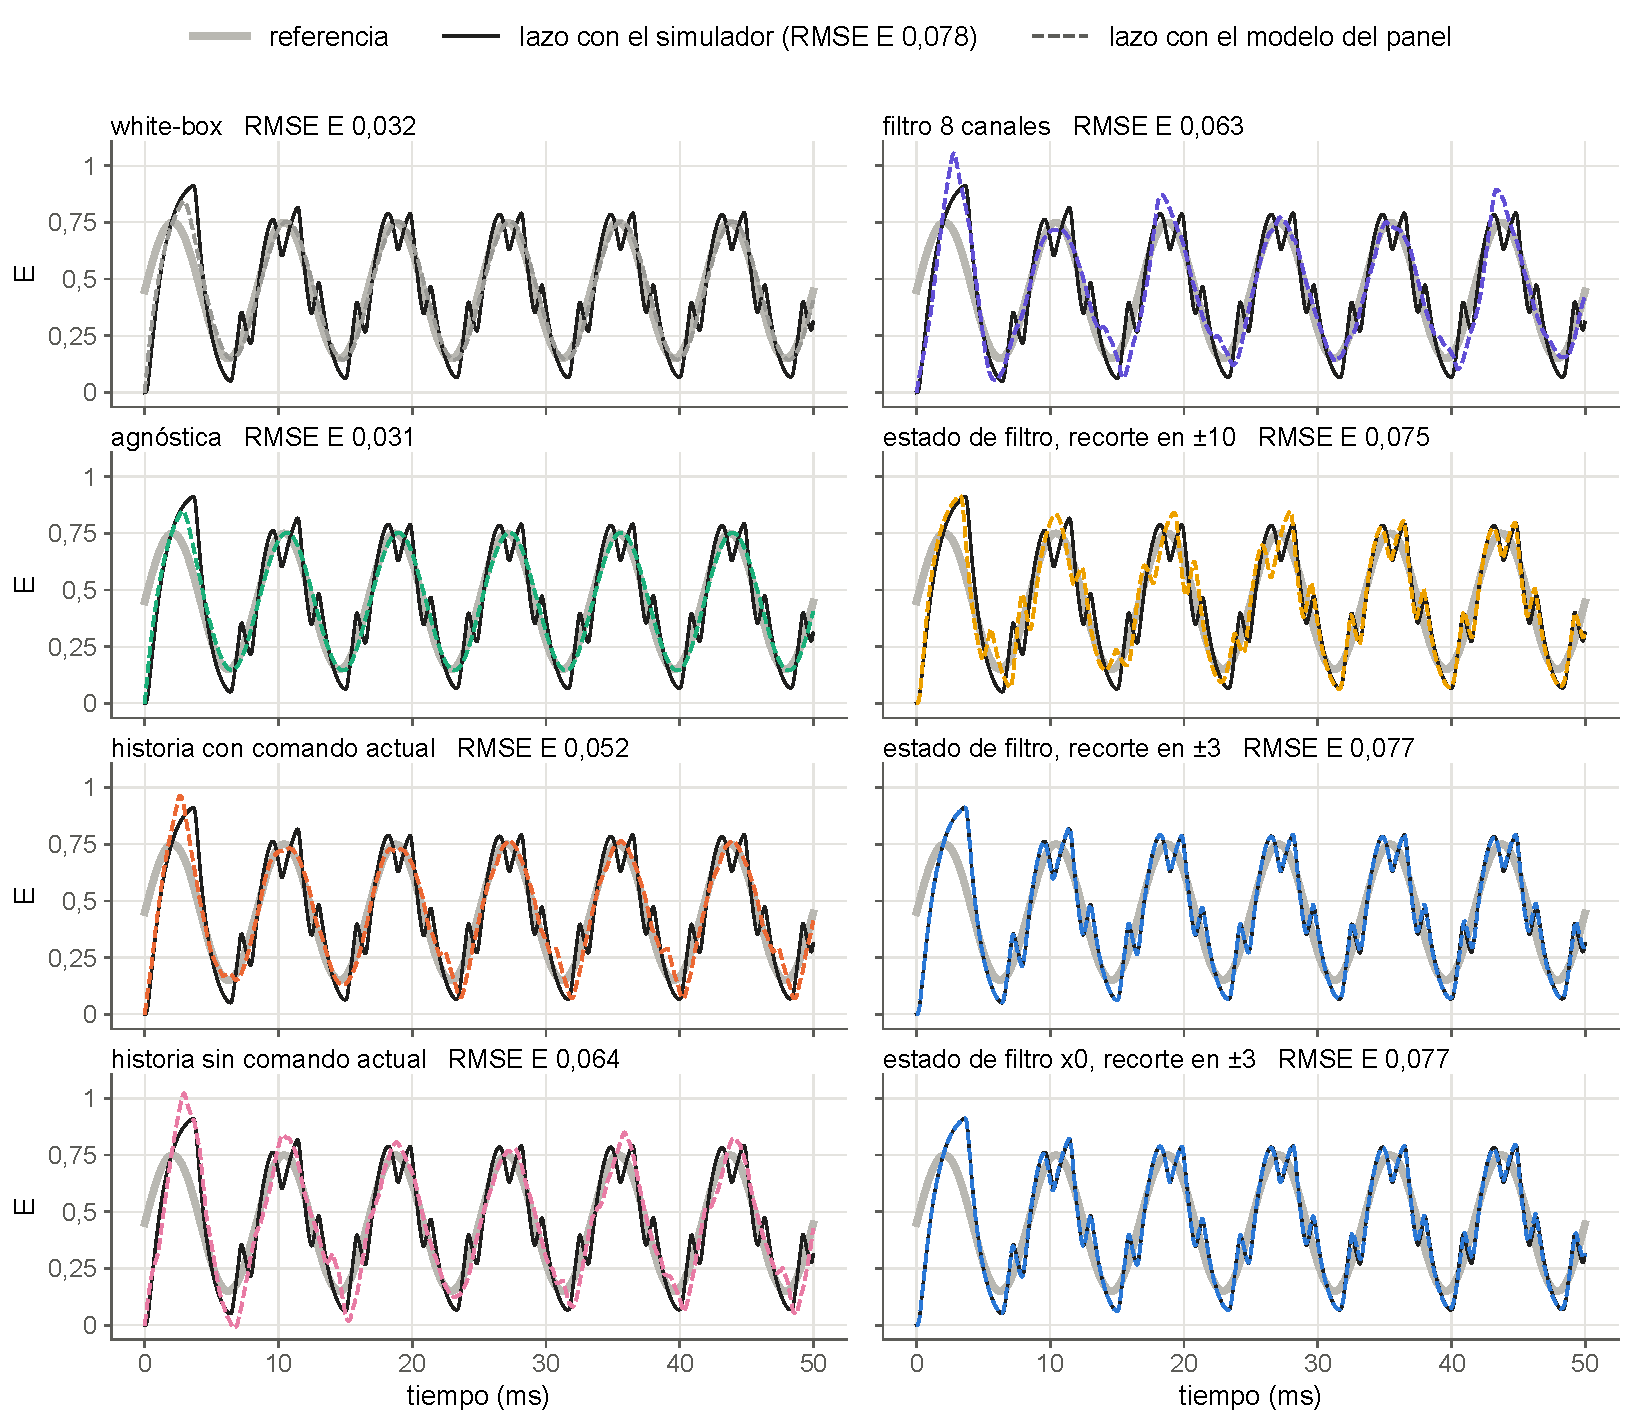
\includegraphics[width=\textwidth]{gamma50_E.pdf}
\caption{Actividad excitatoria $E$ con la gamma continua de 50~ms. Gris, referencia. Negro, lazo con el simulador. Discontinua, lazo con el modelo del panel.}
\end{figure}
\begin{figure}[H]
\centering
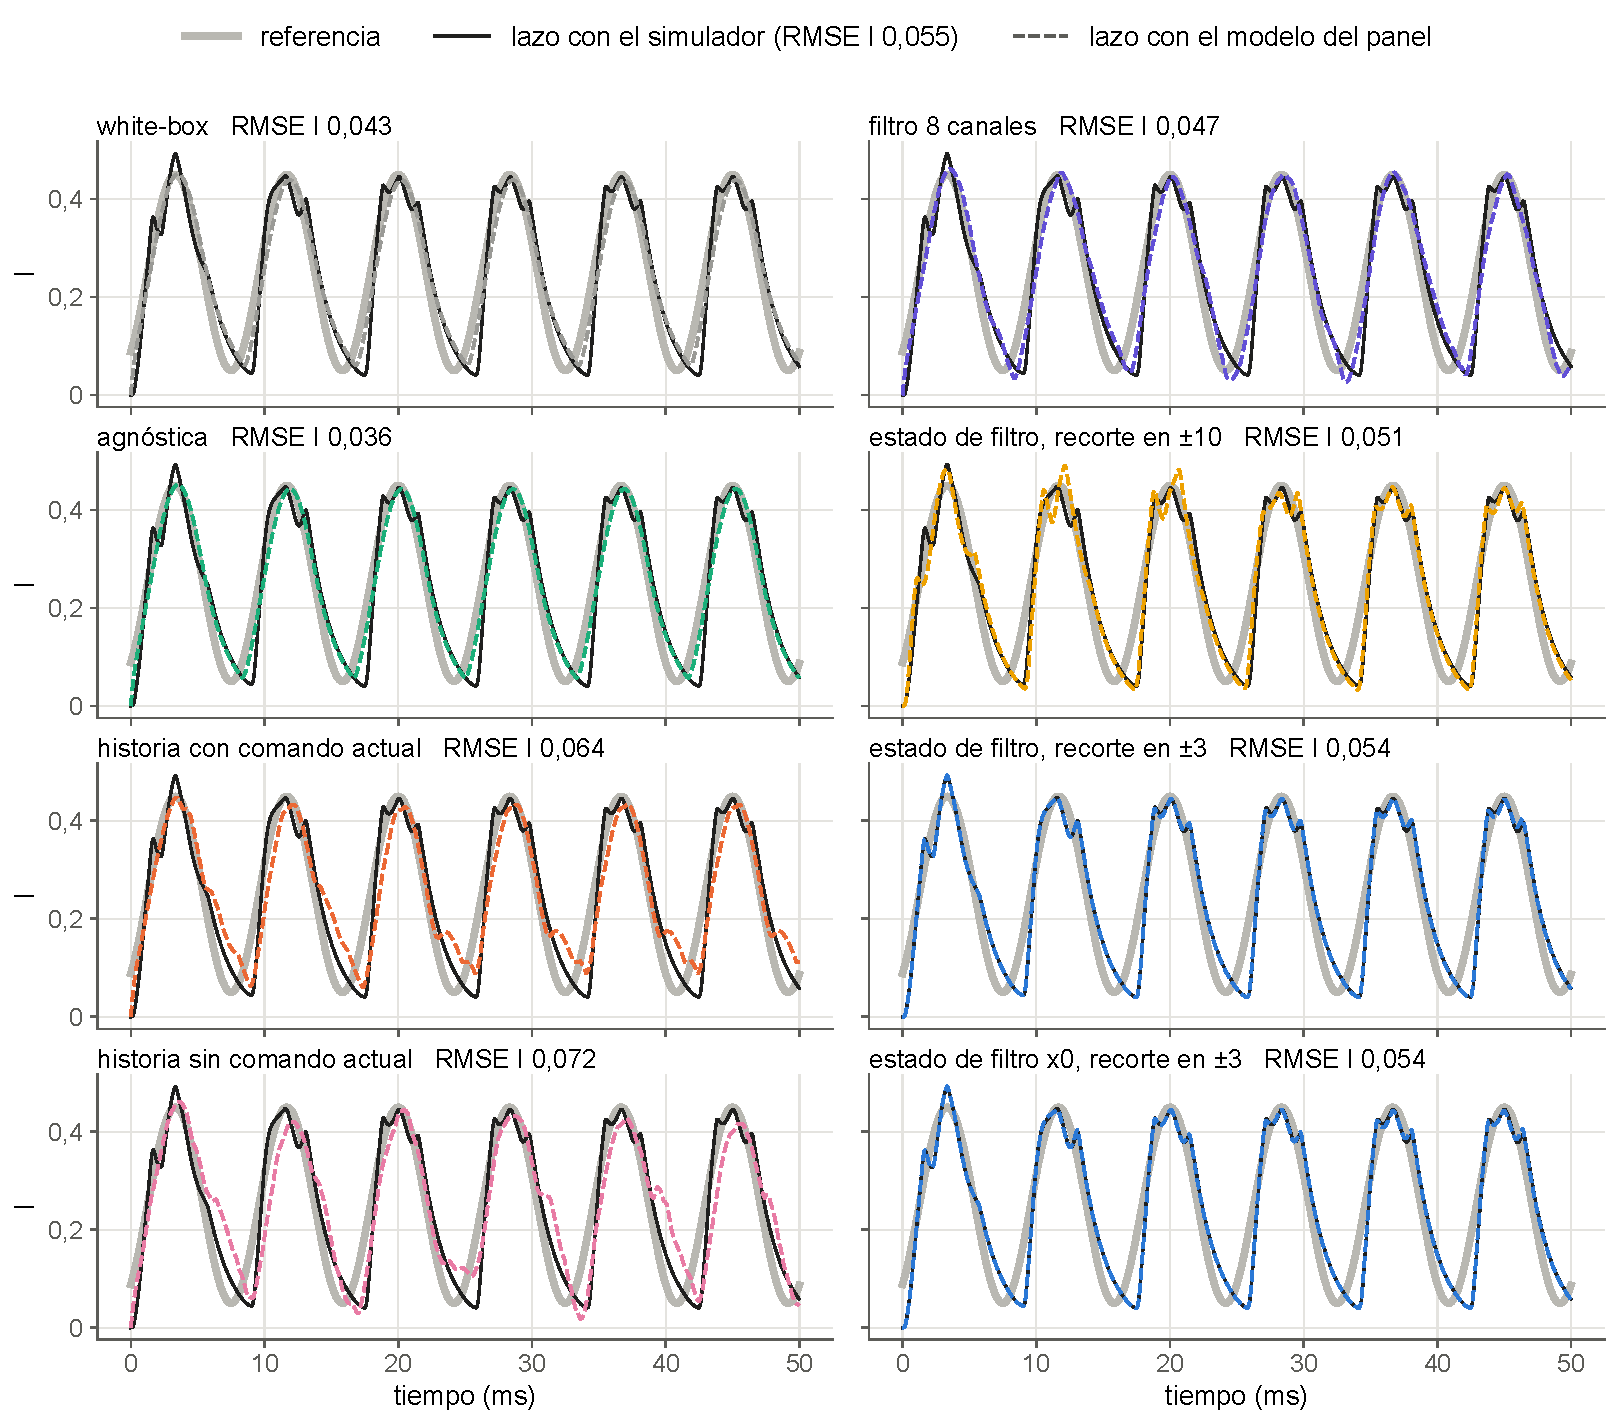
\includegraphics[width=\textwidth]{gamma50_I.pdf}
\caption{Actividad inhibitoria $I$ en las mismas corridas.}
\end{figure}
Con la gamma continua, el lazo con el simulador va atrasado respecto de la referencia, por el filtro del actuador, y su RMSE es 0,068. El white-box y la agnóstica quedan en fase con la referencia (0,038 y 0,034). El estado de filtro con recorte en $\pm 3$ reproduce el atraso del simulador. Las correcciones con historia quedan entre 0,056 y 0,069, con la forma de onda de $I$ deformada en los valles.


\subsection{Referencias con el comando en el rango de entrenamiento}

Referencia: $\big(r_I(t), r_E(t)\big) = \big(I(t), E(t)\big)$, la solución del Wilson-Cowan sin perturbación desde el reposo con
\[
P(t) = 1 + 0{,}8\,\sin(2\pi f t), \qquad Q(t) = 0{,}75 + 0{,}6\,\sin(2\pi f t - 1),
\]
con $f = 8$~Hz y $t \in [0, 500]$~ms para la theta, y $f = 40$~Hz y $t \in [0, 250]$~ms para la gamma.

\begin{figure}[H]
\centering
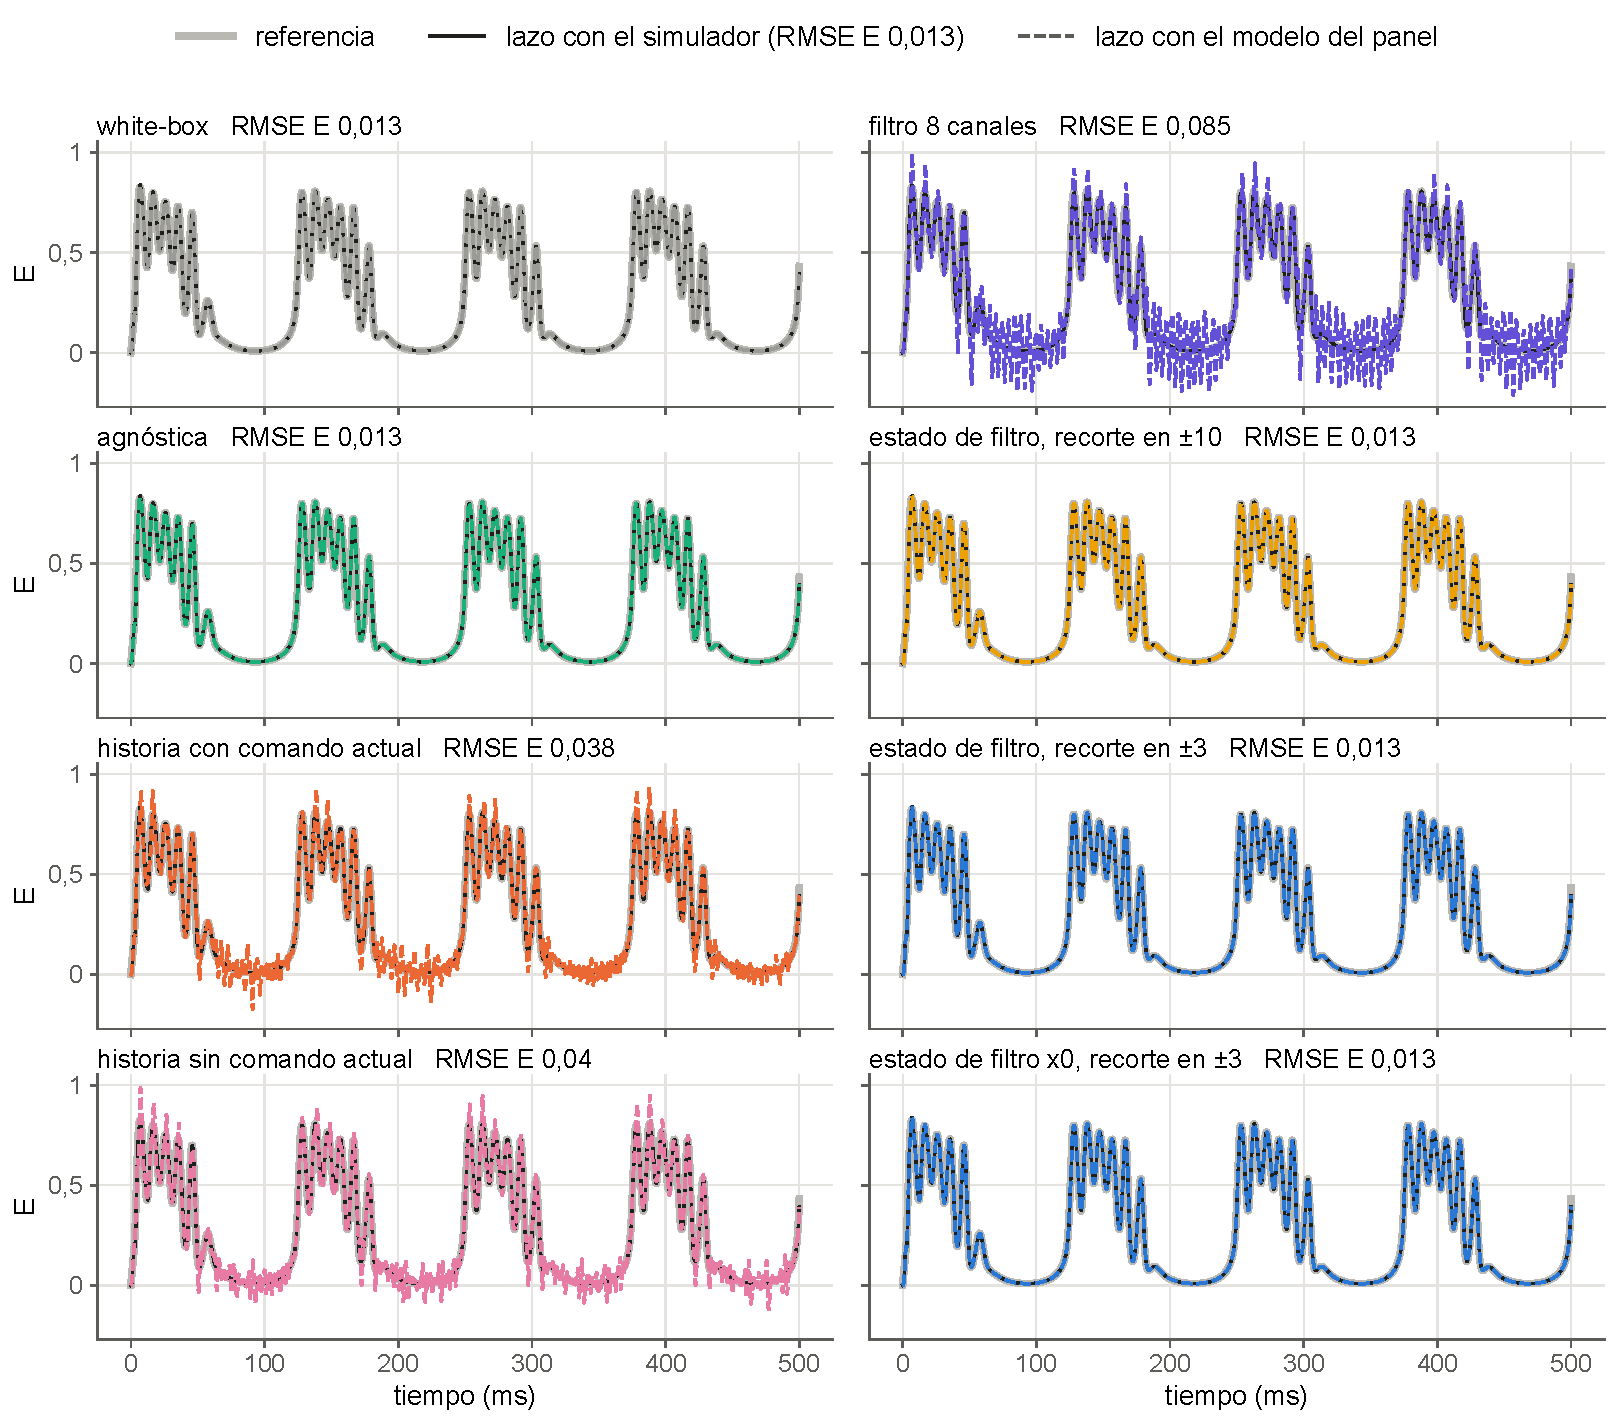
\includegraphics[width=\textwidth]{theta_rango_E.pdf}
\caption{Actividad excitatoria $E$ con la referencia theta de 8~Hz en rango, 500~ms.}
\end{figure}
\begin{figure}[H]
\centering
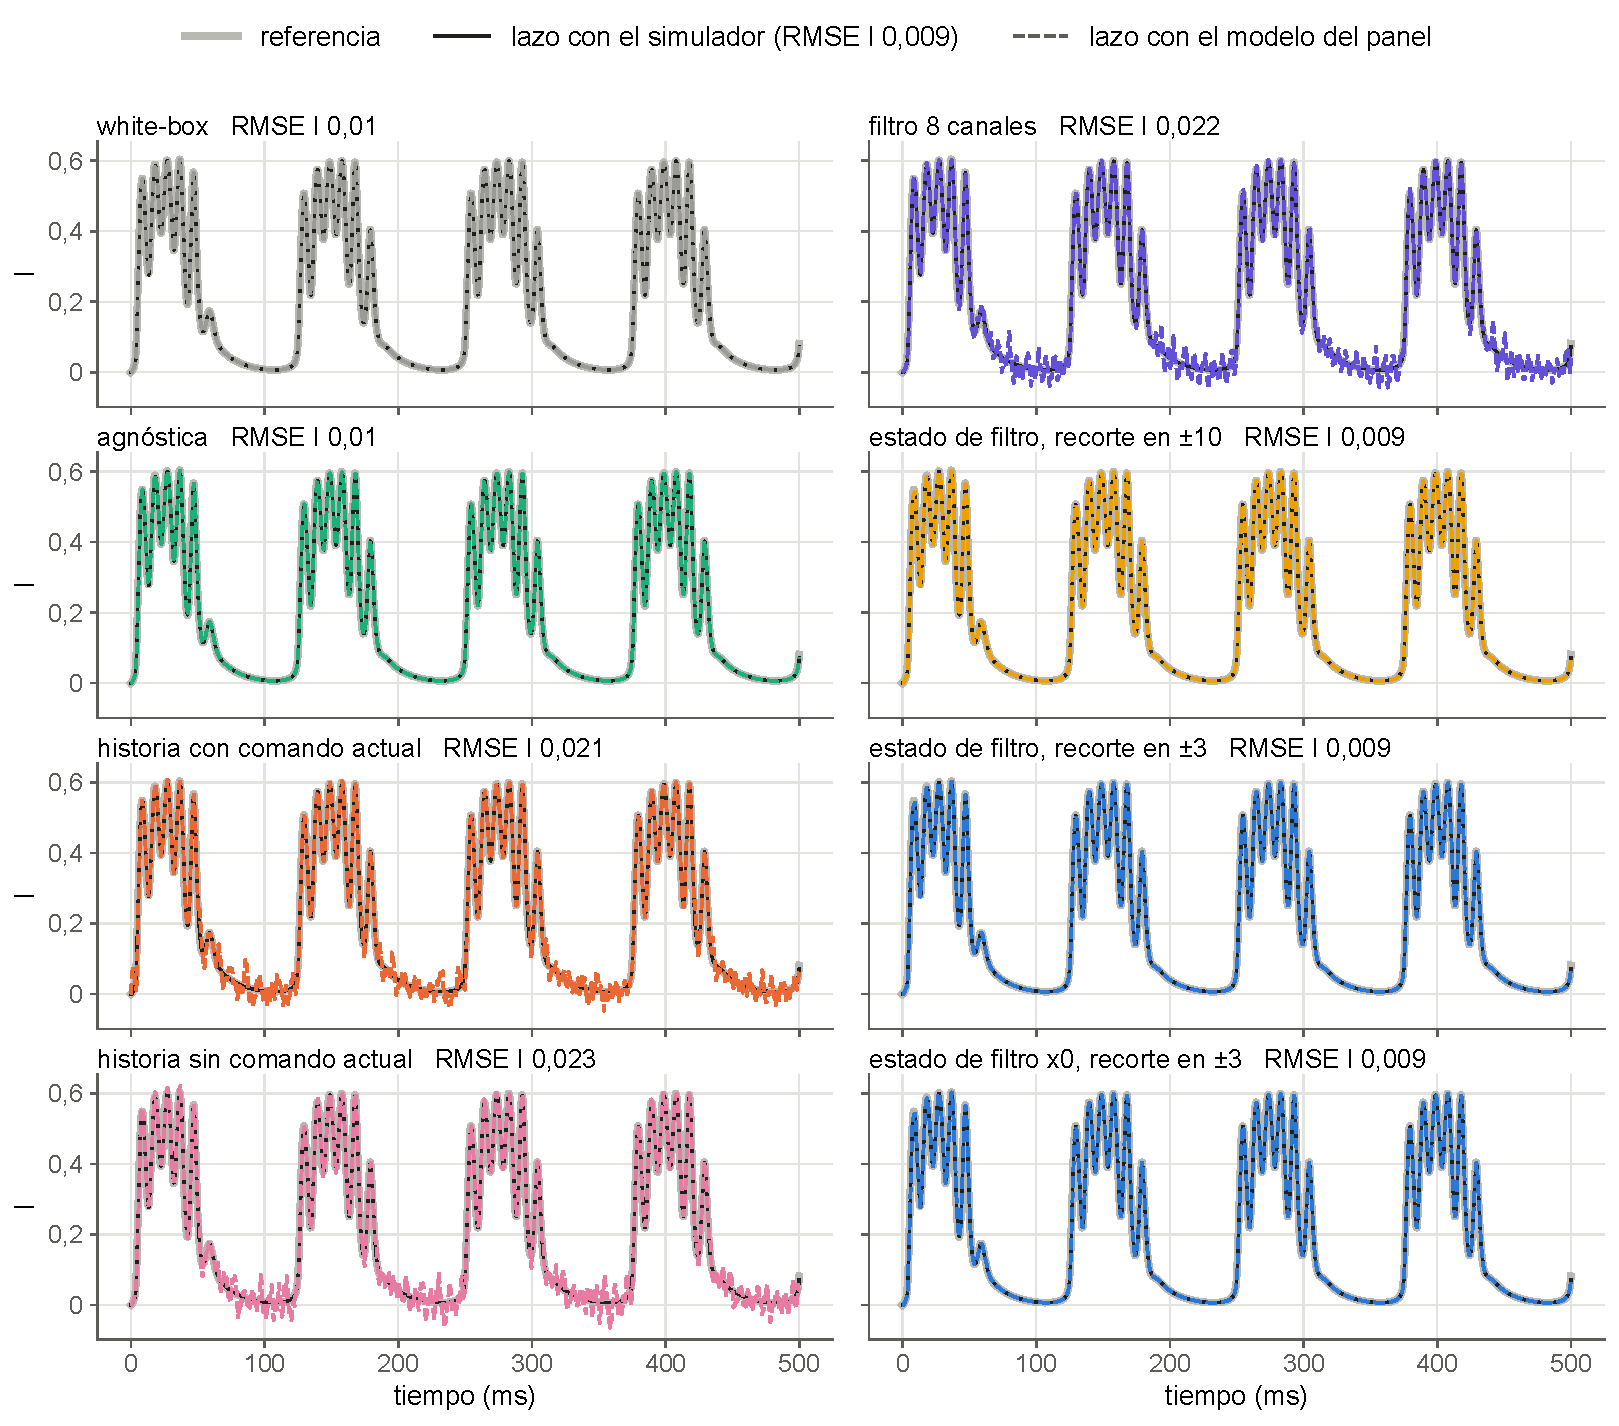
\includegraphics[width=\textwidth]{theta_rango_I.pdf}
\caption{Actividad inhibitoria $I$ con la referencia theta de 8~Hz en rango.}
\end{figure}
\begin{figure}[H]
\centering
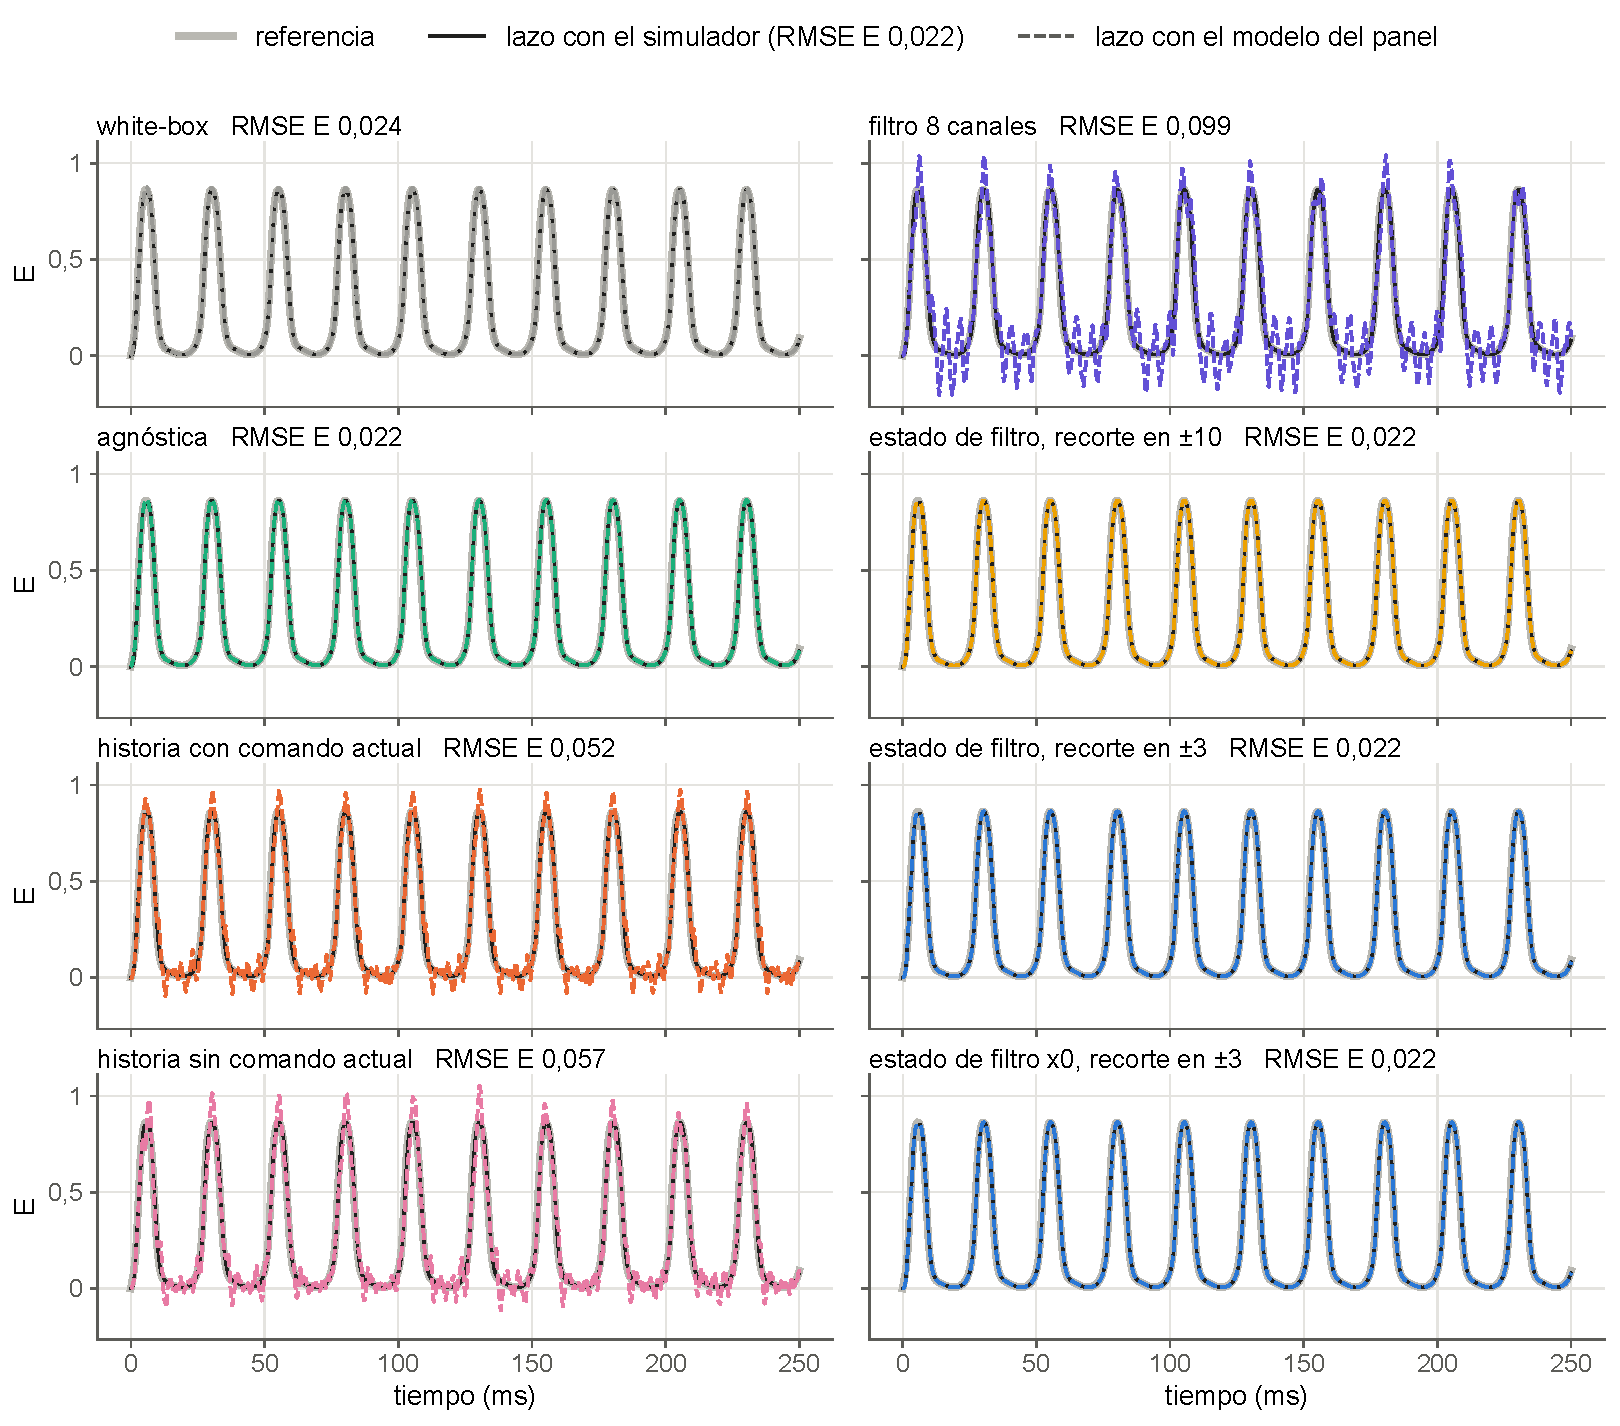
\includegraphics[width=\textwidth]{gamma_rango_E.pdf}
\caption{Actividad excitatoria $E$ con la referencia gamma de 40~Hz en rango, 250~ms.}
\end{figure}
\begin{figure}[H]
\centering
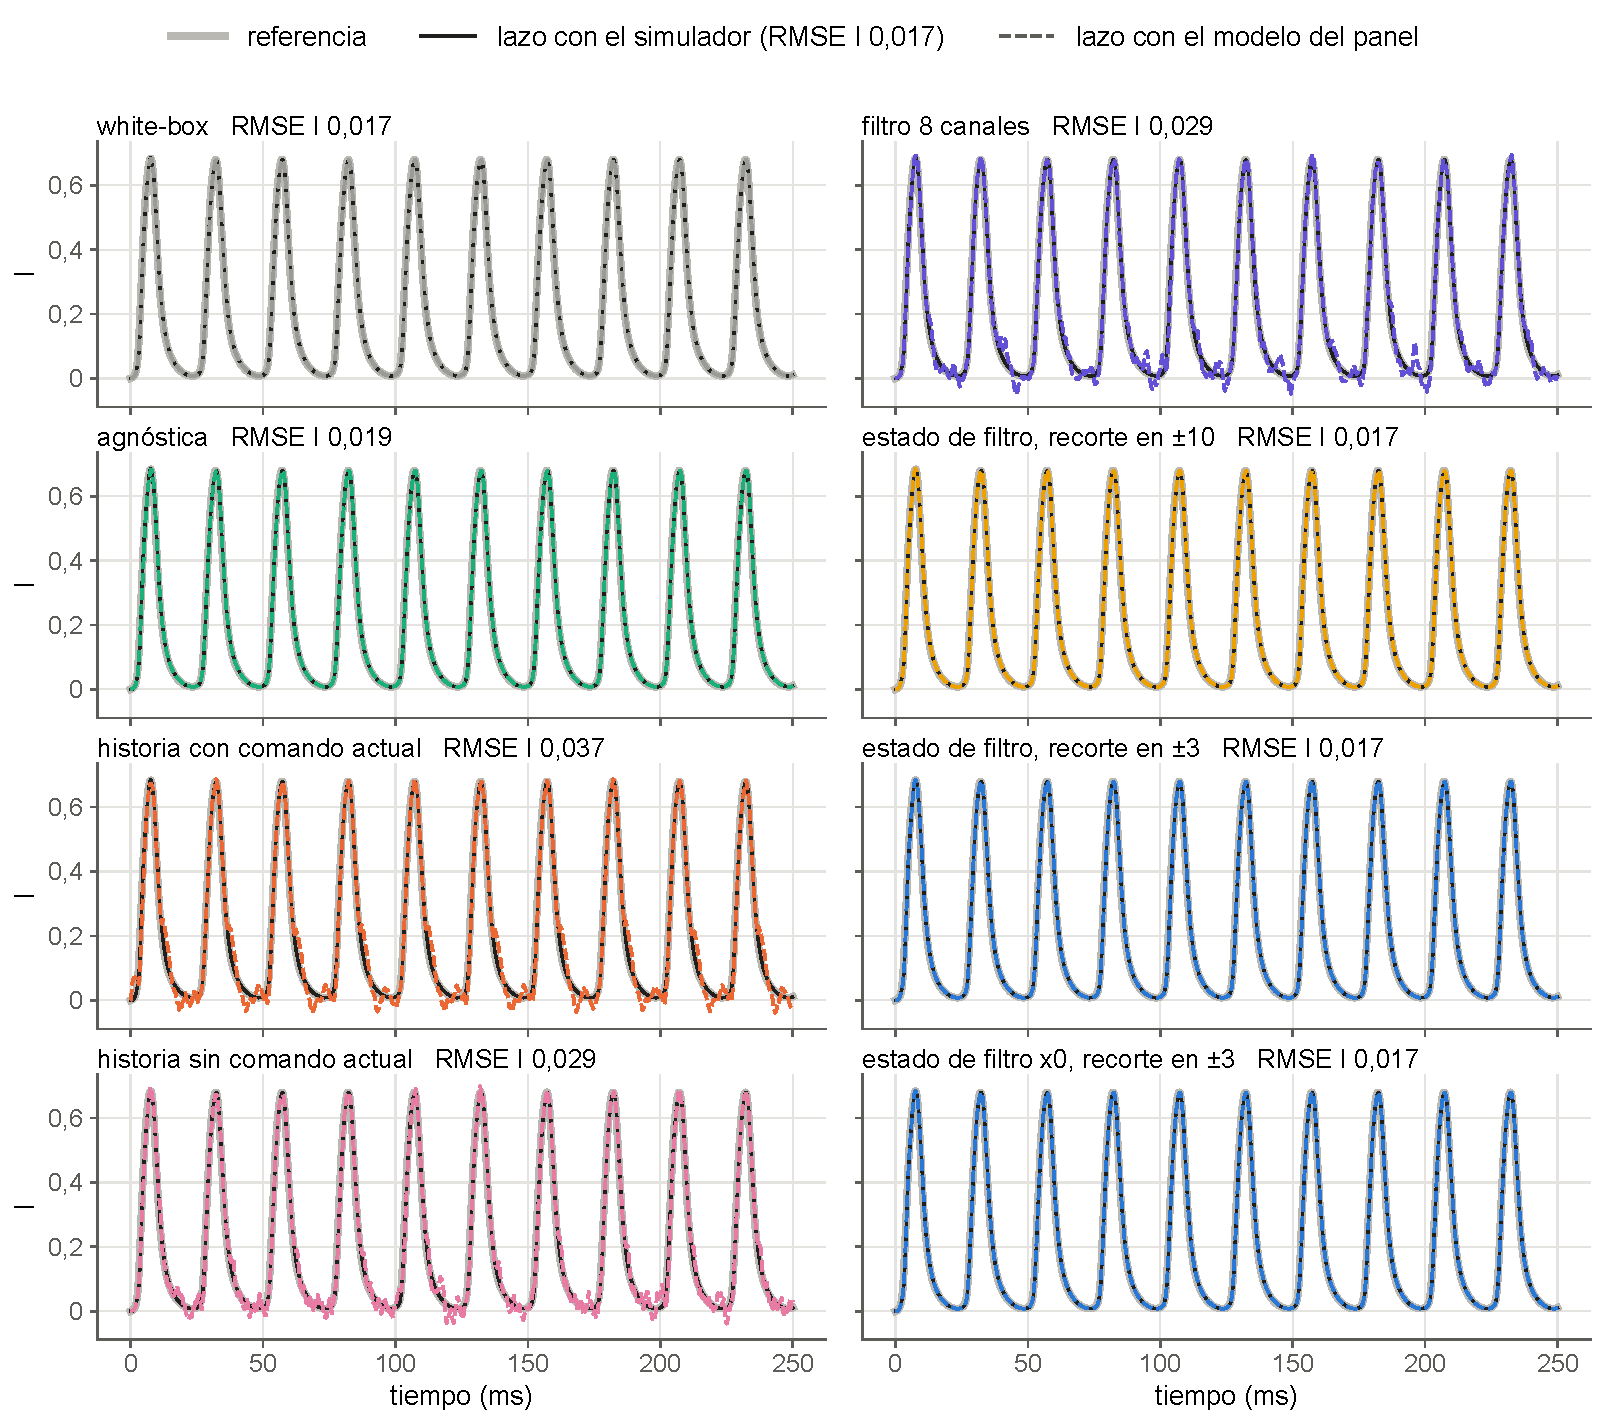
\includegraphics[width=\textwidth]{gamma_rango_I.pdf}
\caption{Actividad inhibitoria $I$ con la referencia gamma de 40~Hz en rango.}
\end{figure}
Con estas referencias el lazo con el simulador sigue con RMSE de 0,011 (theta) y 0,020 (gamma), y su comando queda dentro de $[0, 2]$ el 99~\% del tiempo. El white-box, la agnóstica y las tres versiones del estado de filtro reproducen ese seguimiento. Las correcciones con historia oscilan en los tramos de baja actividad, y su RMSE es de 2 a 5 veces el del lazo con el simulador. En sus lazos el comando sale de $[0, 2]$ entre el 45 y el 80~\% del tiempo, aunque la referencia no lo pide. La salida del rango la produce el propio lazo con el modelo. Un error chico de la red cerca del reposo, donde la sigmoidea es plana, se convierte en un comando grande, y ese comando, fuera del rango de entrenamiento, vuelve a entrar a la red.


\section{RMSE contra la referencia}

RMSE contra la referencia, combinado como $\sqrt{(e_I^2 + e_E^2)/2}$, sobre el último 80~\% de cada corrida. Semilla 0, $\sigma = 0{,}01$, simulador con recorte.

\begin{center}
\small
\begin{tabular}{@{}lcccc@{}}
\toprule
planta en el lazo & theta-gamma & gamma 50~ms & theta en rango & gamma en rango \\
\midrule
simulador & 0,057 & 0,068 & 0,011 & 0,020 \\
white-box & 0,045 & 0,038 & 0,011 & 0,021 \\
agnóstica & 0,044 & 0,034 & 0,011 & 0,021 \\
historia con comando actual & 0,061 & 0,058 & 0,031 & 0,045 \\
historia sin comando actual & 0,070 & 0,069 & 0,033 & 0,045 \\
filtro 8 canales & 0,089 & 0,056 & 0,062 & 0,073 \\
estado de filtro, recorte en ±10 & 0,056 & 0,064 & 0,011 & 0,020 \\
estado de filtro, recorte en ±3 & 0,057 & 0,066 & 0,011 & 0,020 \\
estado de filtro x0, recorte en ±3 & 0,057 & 0,066 & 0,011 & 0,020 \\
\bottomrule
\end{tabular}
\end{center}


\end{document}
